\documentclass{article}
\setcounter{secnumdepth}{2}

%% Packages -------------------------------------------------------------------
\RequirePackage[english]{babel} % Document's language
\RequirePackage[utf8]{inputenc} % Special characters
\RequirePackage[section]{placeins}%Pour placement de section
\RequirePackage[T1]{fontenc} %Quelques lettres qui sont pas inclus dans UTF-8
\RequirePackage{mathtools} %Paquet pour des équations et symboles mathématiques
\RequirePackage{siunitx} %Pour écrire avec la notation scientifique (Ex.: \num{2e+9})
\usepackage{amsmath}
\usepackage{amssymb}
\RequirePackage{float} %Pour placement d'images
\RequirePackage{graphicx} %Paquet pour insérer des images
\RequirePackage[justification=centering]{caption} %Pour les légendes centralisées
\RequirePackage{subcaption}
\RequirePackage{wallpaper}
\RequirePackage{nomencl}
%\makenomenclature
\RequirePackage{fancyhdr}
%\pagestyle{fancy}
%\fancyheadoffset{1cm}
%\setlength{\headheight}{2cm}
\RequirePackage{url}
\RequirePackage[hidelinks]{hyperref}%Paquet pour insérer légendes dans des sous-figures comme Figure 1a, 1b
\RequirePackage[left=2.5cm,right=2.5cm,top=2cm,bottom=3.5cm]{geometry} %Configuration de la page
\usepackage{ragged2e}
\usepackage{blindtext}
\usepackage{qtree}


\begin{document}

\begin{titlepage}
\centering


\includegraphics[width=0.5\textwidth]{imgs/mva.png}
\par\vspace{1cm}

{\scshape\LARGE Rémi Ouazan \\ Optimal Transport \par} 
\vspace{0.5cm}

\rule{\linewidth}{0.2 mm} \\[0.4 cm]
{\huge\bfseries Project 46 : Flowtree \par} \
\rule{\linewidth}{0.2 mm} \\[1.0 cm]

\section*{Abstract}

\justifying
Coucou c'est moi l'abstract!

\vfill

\centering
{\large January 2023\par} %Affichage de la date

\end{titlepage}

\newpage
\section{Flowtree algorithm}
In the following we'll assume $X$ is in $\mathbb{R}^d_+$, which we can ensure with an affine transform, that doesn't affect distances.  We'll also note $\Phi = \text{max}(\Vert x_1 \Vert_\infty, \dots, \Vert x_n \Vert_\infty)$, thus $X \in [0, \Phi]^d$. The aim of this algorithm is finding an approximate of $W_1$ for two distributions $\mu$ and $\nu$ defined on $X$.

\subsection{Building the quadtree}\label{ssec:building_the_quandtree}
Step 1 in the Flowtree algorithm is to build a quadtree $Q(X)$ from $X$. $Q(X)$ is a tree that will help us compute an approximation of the Wassertein-1 distance quickly.

In this step, the notion of \textbf{hypercube} is quite important. With say that $H$ is a $d$ dimensionnal hypercube if $\exists (x, l) \in \mathbb{d} \times \mathbb{R}_+$ such that:

$$
H(x, l) = [x_1, x_1 + l] \times \dots \times [x_d, x_d + l]
$$

We'll call $x$ the corner of the hypercube and $l$ the side length of the hypercube. With $d=2$ we get a square and with $d=3$ a cube. As these examples suggest, hypercube are naturaly recursive: if we consider $H(x, l)$, then there is exactly one way to partition it into $2^d$ hypercubes of side length $l/2$. These sub-hypercubes are of the form:

$$
H(x_{b_1...b_d}, l/2) = [x_1 + b_1 \frac{l}{2}, x_1 + (b_1+1) \frac{l}{2}] \times \dots \times [x_d + b_d \frac{l}{2}, x_d + (b_d+1) \frac{l}{2}]
$$

where $b_1...b_d \in \{ 0, 1 \}^d$. We can call this operation \textbf{splitting} $H$ into sub-hypercubes $H_{0...0}, \dots, H_{1...1}$.\\

We can now begin building $Q(X)$. We compute $\sigma$ a random vector where each component is i.i.d. in $\mathcal{U}(0, \Phi)$ and define $H_0 = [-\Phi, \Phi]^d + \sigma$. Remark that $H_0$ contains $X$ and has side length $2\Phi$. We define the root of $Q(X)$ as the node associated with $H_0$. We then split $H_0$ into $2^d$ sub-hypercubes. For each sub-hypercube $H$, there are 3 cases. If $H \cap X = \emptyset$ then $H$ is discarded. If $H \cap X = \{x_i\}$ then we attach a leaf $(i)$ to the root and discard $H$. Otherwise $H \cap X$ contains multiple elements of $X$ and we attach a node associated with $H$ to the root, and repeat this process on that node.\\
Since $X$ is finite, the tree building finishes. Furthermore, the tree has exactly one leaf per element of $X$. The process in 2D can be seen in figure \ref{quadtree}.

\begin{figure}[h]
\centering
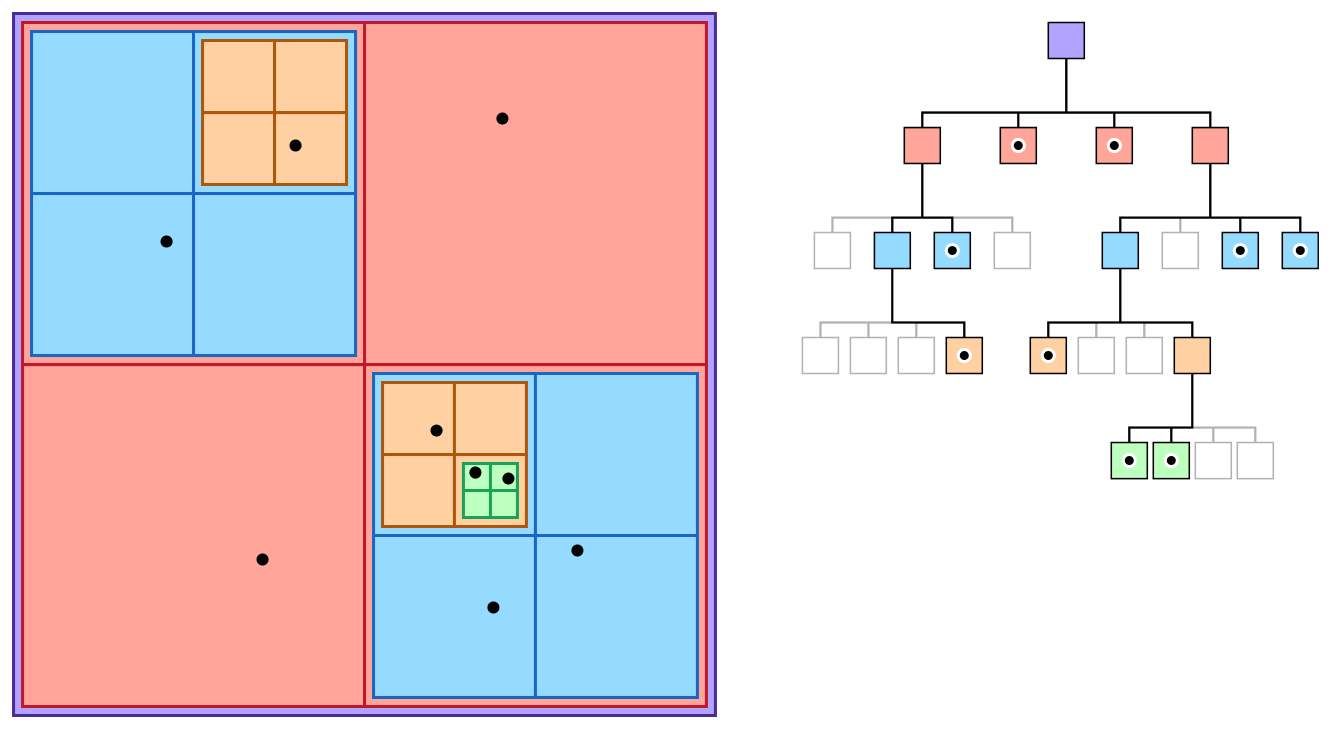
\includegraphics[width=0.7\textwidth]{imgs/quadtree.png}
\caption{A 2D quadtree \textit{(source: Apple)}}
\label{quadtree}
\end{figure}

To define a distance on $Q(X)$, we say that the edge between a node of depth $d$ and a node of depth $d+1$ has weight $2^{\log(\Phi)-d}$. We consider the root to be of depth $0$, thus the edges between the root and its children have weight $2^{\log(\Phi)}$. The distance $t$ between two leaves is then defined as the sum of the weights of each edges present along the unique path between the two leaves.
%TODO Why that's a good approximation of the L1 distances

Interestegly, this step doesn't involve the distributions $\mu$ and $\nu$ for which we intend to compute an estimate of $W_1$. We can build the quadtree on $X$ and repeat the steps 2 and 3 for any number of distributions, which is why this algorithm is used for neireast neighboor search. 

\subsection{Computing the optimal flow}
Step 2 of the flowtree is computing the solution of Kantorovitch problem in regards to $Q(X)$, $\mu$ and $\nu$:

$$
f^* = \underset{f \in \mathcal{M}(\mu, \nu)}{\text{argmin}} \sum_{(x, x') \in Q(X)^2} t(x, x') f(x, x')
$$

where $\mathcal{M}(\mu, \nu) = \lbrace f \in \mathcal{M}_+(X, X),~ p_1(f) = \mu,~ p_2(f) = \nu \rbrace$ is the set of distributions over $X^2$ with $\mu$ and $\nu$ as marginals. The elements of this set are called \textbf{flows} and $f^*$ is the \textbf{optimal flow}.\\
Here lies the interest of $Q(X)$, because $f^*$ can be computed exaclty with complexity $\mathcal{O}(s(d+h))$ where $h$ is the height of $Q(X)$ and $s$ is an upper bound for the size of the supports $\mu$ and $\nu$. This exact computation is quite rare for Kantorovitch problem as REF shows.\\

To do this, we first turn $Q(X)$ into a tree $D(X, \mu, \nu)$ that we'll call the demand tree, for reasons that will become apparent later. We define $D(X, \mu, \nu)$ by taking $Q(X)$ structure (we leave all nodes intact) and replacing the content of each leaf. Recall each leaf has an index $(i)$ because it corresponds to an element $x_i$ of $X$. Leaf $(i)$ in the quadtree becomes leaf 
$\left( \lbrace \mu_i \triangleq \mu(x_i) \rbrace , \lbrace \nu_i \triangleq \nu(x_i) \rbrace \right)$ 
in the demand tree. We call set $\lbrace \mu_i \rbrace$ the $\mu$-demand and same goes for $\nu$. This process is visible in figure REFQtree2Dtree.

\centering
\begin{tabular}{lll}

\Tree[.$Q(X)$ [. [.2 ]
               [.5 ]]
            [. [.1 ]
               [.  [
               	   [.3 ]
               	   [.4 ]]]]]
               	   
&    

\begin{tabular}{ |c|ccccc| } 
\hline
k & 1 & 2 & 3 & 4 & 5 \\ 
\hline
$\mu(k)$ & 0.1 & 0.2 & 0 & 0.2 & 0.5 \\ 
\hline
$\nu(k)$ & 0.5 & 0.2 & 0 & 0 & 0.3 \\ 
\hline
\end{tabular}

&

\Tree[.{$D(X, \mu, \nu)$} [. [.{$\mu_2 = 0.2$ \\ $\nu_2 = 0.2$} ]
               [.{$\mu_5 = 0.5$ \\ $\nu_5 = 0.3$} ]]
            [. [.{$\mu_1 = 0.1$ \\ $\nu_1 = 0.4$} ]
               [. [. {$\emptyset$} ]
               	  [.{$\mu_4 = 0.2$ } ]]]]
               		
\end{tabular}

\justifying
In practice, since the support of $\mu$ and $\nu$ are bounded by $s$, 
many of these leaves become leaf $(\emptyset, \emptyset)$, 
as is the case with leaf $(3)$ in figure REFQtree2Dtree. 
To compute the optimal flow, we begin with an emtpy flow $f=0$. We then traverse the demand tree in postorder, which means that we only visit a node after passing through all of its children. When visiting node $N$:

\begin{enumerate}

\item If node $N = (N_\mu, N_\nu)$ is equal to $(\emptyset, \cdot)$ or $(\cdot, \emptyset)$, we stop there and kick the (eventual) remaining demand to the parent node.

\item Since the $\mu$-demand $N_\mu$ (resp. the $\nu$-demand $N_\nu$) isn't empty, $\exists i$ (resp. $j$) such that $\mu_i = \min N_\mu$ (resp. $\nu_j = \min N_\nu$). We compute these indices and the quantity $d = \min (\mu_i, \nu_j)$.

\item We then update the demand of node $N$ with $\mu_i := \mu_i - d$ and $\nu_j := \nu_j - d$ 

\item We update the flow with $f(x_i, x_j) := f(x_i, x_j) + d$.

\item Go back to step 1.

\end{enumerate}

To understand this algorithm, it helps to think in term of offer and demand. Say $\mu$ is the distribution of producers of a goods (offer) and $\nu$ is the distribution of demanders of goods (demand). If offer and demand exist in the same place, ie on the same node, then we can do the exchange in that place (step 4) and we keep track of the exchange made (step 5). This exchange has to be small enough for both the producer and the demander, thus we look for the minimal exchange (step 3). Otherwise (stop case of step 1), we have to move the goods, which corresponds to kicking the demand (both in term of producers and demanders) to the parent node.\\
In this example, the $\mu$-demand is called the offer and the $\nu$-demand the demand, but in the general case, both are called demands. One can think of the $\mu$-demand (the offer) as a demand for buyers, and the $\nu$-demand (the demand) as a demand for sellers. \\
To illustrate this algorithm, we can refer to table \ref{table:flow_computation}.

\begin{table}[H]
\centering
\begin{tabular}{c|c} 
\Tree[.{$D(X, \mu, \nu)$} [. [.{$\mu_2 = 0.2$ \\ $\nu_2 = 0.2$} ]
                             [.{$\mu_5 = 0.5$ \\ $\nu_5 = 0.3$} ]]
                          [. [.{$\mu_1 = 0.1$ \\ $\nu_1 = 0.5$} ]
                             [.  [
               	                 [.{$\emptyset$} ]
               	                 [.{$\mu_4 = 0.2$} ]]]]]
&
\hspace{20pt} ~
\Tree[.{$D(X, \mu, \nu)$} [. [.{$\emptyset$} ]
                             [.{$\mu_5 = 0.2$} ]]
                          [. [.{$\nu_1 = 0.4$} ]
                             [.  [
               	                 [.{$\emptyset$} ]
               	                 [.{$\mu_4 = 0.2$ } ]]]]]
\\
\begin{tabular}{ |c|ccccc| } \hline
f & 1 & 2 & 3 & 4 & 5 \\ \hline
1 & 0 & 0 & 0 & 0 & 0 \\ 
2 & 0 & 0 & 0 & 0 & 0 \\ 
3 & 0 & 0 & 0 & 0 & 0 \\ 
4 & 0 & 0 & 0 & 0 & 0 \\ 
5 & 0 & 0 & 0 & 0 & 0 \\ \hline \end{tabular} 
&
\begin{tabular}{ |c|ccccc| } \hline
f & 1 & 2 & 3 & 4 & 5 \\ \hline
1 & 0.3 & 0 & 0 & 0 & 0 \\ 
2 & 0 & 0.2 & 0 & 0 & 0 \\ 
3 & 0 & 0 & 0 & 0 & 0 \\ 
4 & 0 & 0 & 0 & 0 & 0 \\ 
5 & 0 & 0 & 0 & 0 & 0.3 \\ \hline \end{tabular} \\
\\ \hline \\
\Tree[.{$D(X, \mu, \nu)$} [. {$\mu_5 = 0.2$} ]
                          [. {$\mu_4 = 0.2$ \\ $\nu_1 = 0.4$} ]]
\hspace{18pt} ~~
&
\Tree[.{$D(X, \mu, \nu)$} [. {$\mu_5 = 0.2$} ]
                          [. {$\nu_1 = 0.2$} ]]
\hspace{15pt} ~
\\
\begin{tabular}{ |c|ccccc| } \hline
f & 1 & 2 & 3 & 4 & 5 \\ \hline
1 & 0.3 & 0 & 0 & 0 & 0 \\ 
2 & 0 & 0.2 & 0 & 0 & 0 \\ 
3 & 0 & 0 & 0 & 0 & 0 \\ 
4 & 0 & 0 & 0 & 0 & 0 \\ 
5 & 0 & 0 & 0 & 0 & 0.3 \\ \hline \end{tabular}
&
\begin{tabular}{ |c|ccccc| } \hline
f & 1 & 2 & 3 & 4 & 5 \\ \hline
1 & 0.3 & 0 & 0 & 0 & 0 \\ 
2 & 0 & 0.2 & 0 & 0 & 0 \\ 
3 & 0 & 0 & 0 & 0 & 0 \\ 
4 & 0.2 & 0 & 0 & 0 & 0 \\ 
5 & 0 & 0 & 0 & 0 & 0.3 \\ \hline \end{tabular} \\
\\ \hline \\
\Tree[.{$D(X, \mu, \nu)$} [. {$\mu_5 = 0.2$ \\ $\nu_1 = 0.2$ } ]] \hspace{25pt} ~~
&
\Tree[.{$D(X, \mu, \nu)$} [. {$\emptyset$} ]] \hspace{18pt} ~~
\\
\begin{tabular}{ |c|ccccc| } \hline
f & 1 & 2 & 3 & 4 & 5 \\ \hline
1 & 0.3 & 0 & 0 & 0 & 0 \\ 
2 & 0 & 0.2 & 0 & 0 & 0 \\ 
3 & 0 & 0 & 0 & 0 & 0 \\ 
4 & 0.2 & 0 & 0 & 0 & 0 \\ 
5 & 0 & 0 & 0 & 0 & 0.3 \\ \hline \end{tabular}
&
\begin{tabular}{ |c|ccccc| } \hline
f & 1 & 2 & 3 & 4 & 5 \\ \hline
1 & 0.3 & 0 & 0 & 0 & 0 \\ 
2 & 0 & 0.2 & 0 & 0 & 0 \\ 
3 & 0 & 0 & 0 & 0 & 0 \\ 
4 & 0.2 & 0 & 0 & 0 & 0 \\ 
5 & 0.2 & 0 & 0 & 0 & 0.3 \\ \hline \end{tabular}
               		
\end{tabular}
\caption{Optimal flow computation for the demand tree described in REF}
\label{table:flow_computation}
\end{table}

Although we written the $\mu$-demand as a set $\lbrace \mu_i, \dots \rbrace$ to save time, we do need to keep track of both $i$ and the associated quantity $\mu_i$. More on that in part REF. 

\subsection{Compute $W_1$ estimate}
We now compute the $W_1$ estimate using the optimal flow $f^*$ computed on $D(X, \mu, \nu)$. The logic here is that since $f^*$ is the optimal argument to the Kantorovitch problem defined by the tree distance, itself an approximation of the $l_1$ distance, then using $f^*$ as an argument for the Kantorovitch problem defined by the $l_1$ distance will yield a near-optimal value.\\

This final step is quite simple: we just have to sum over the couples for which $f^*$ is non-zero the optimal flow value times the distance of the two points to get the estimate $\widetilde{W}_1$ of $W_1$:

$$
\widetilde{W}_1(\mu, \nu) = \sum_{(x, x') \in S^*} f^*(x, x') \Vert x - x' \Vert_2
$$ %TODO Talk about norm 2

with $S^*$ the support of $f^*$.

\section{Technical details}

\subsection{Fusing step 2 and 3} \label{ssec:fuse23}
Since the only use of $f^*$ is to be used for the computation of $\widetilde{W}_1(\mu, \nu)$, one can fuse the step 2 and 3 of the algorithm by not computing $f^*$ but incrementaly increasing $\widetilde{W}_1(\mu, \nu)$ during step 2. We remove step 3 and replace at sub-step of step 2:

4. We update the flow with $f(x_i, x_j) := f(x_i, x_j) + d$.
\\
with:

4. We update the estimate with $\widetilde{W}_1(\mu, \nu) := \widetilde{W}_1(\mu, \nu) + d \Vert x_i - x_j \Vert_2 $.
\\
We can go further add memoïze the distances $\Vert x_i - x_j \Vert_2$ as we compute them and decrease the computationnal cost (by increasing the memory cost).

\subsection{Data structures}
As we mentionned ealrier, given a node $N$ with $\mu$-demand and $\nu$-demand, we need to keep track of $i$ and $\mu_i$ (same goes for $\nu$). Thus, we uset an array with 3 columns: index $i$, $\mu_i$ and $\nu_i$. Each node as an array and the algorithm finishes when the root has been visited and its array is empty. If it isn't, then there was an error during the computation of $f^*$. For instance, this happens if the distribution's masses were not normalized to $1$ or if there is no tolerance for floating-point error. To avoid this, we consider values to be equal to zero when they fall behind $10^{-12}$. Original implemenation REF has $10^{-8}$ but we haven't had any problem with our value.\\ 
For distributions, we used a dictionnary-like data structure that returns $0$ when we try to access a value that isn't in the dictionnary. This is optimal because distributions are only used to access values and check if a value is in the support, both of which are $\mathcal{O}(1)$ operation with dictionnaries.\\
Since we fused step 2 and 3 in subsection \ref{ssec:fuse23}, we need not worry about the data structure of $f^*$, but if for some reason we still wanted to keep the optimal flow (e.g. to try different norms other than the norm 2 in $\widetilde{W}_1$) a dictionnary with default value $0$ is best, as all operations done on it are in $\mathcal{O}(1)$ complexity.

\subsection{Hypercube splitting}
In \ref{ssec:building_the_quandtree}, we defined the split operator on a hypercudbe $H(x, l)$. One can wonder how this is done in practice, as we did when we implemented the Flowtree algorithm. Since we discard the sub-hypercube $H(x_{b_1 \dots b_d}, l/2)$ that intersect no point in $X$, we take advantage of this. We reverse the process: before creating a sub-hypercube, we look if it will contain a point of $X$, and only create it if its the case.\\
Given an hypercube $H(x, l)$ that contains a subset $Y$ of $X$, we compute $m = (x_1+l/2, \dots, x_d+l/2)$ the "middle" of the hypercube. Then, for each $y$ of $Y$, we compute $b = (b_1, \dots, b_d)$ the boolean vector defined by $b_i = 1$ if and only if $y_i \leq m_i = x_i + l/2$. This can be done quickly by rearranging $Y$ into a matrix of dimension $\vert Y \vert \times d$ an do a vectorized comparaison with $m$. 
This results in a boolean matrix $B$ of size $\vert Y \vert \times d$. Each line of $B$ corresponds to a point $y$ and describes the sub-hypercube in which $y$ will be: $y \in H(m + \frac{l}{2}b, l)$.
We have an association from point to sub-hypercube $f: y \rightarrow b$ and need to group points by sub-hypercube. We just reverse $f$ with a dictionnary ($b$ can be stored as bytes to ensure hashability) where keys are $b$ and values $f^{-1}(b)$. This can be done by iterating through the $B$ and costs $(\mathcal{O}\vert Y \vert d)$. Then for each key $b$, if $f^{-1}(b)$ isn't a singleton create an hypercube, otherwise create a leaf.\\

\section{Theoretical garantees}

\subsection{Complexity of Quadtree building}
So as to go with the flow of the paper, we will split the complexiy analysis in two part. As the Flowtree algorithm is meant for nearest neighboor search, the Quadtree $Q(X)$ needs only to be build once, and the computation of $\widetilde{W}_1$ is meant to be repeated for many distributions. Here, we will only cover the cost of buildin $Q(X)$.\\
The paper advertises the cost of building $Q(X)$ as $\widetilde{\mathcal{O}}(\vert X \vert d \log(d\Phi))$. For those unfamiliar with the notation, such as I was, $\widetilde{\mathcal{O}}(n)$ is a shorthand for $\mathcal{O}(n \log(n))$. However, it makes two hypothesis on the data $X$: non-negative coordinates and $\min_{(x, x') \in X^2} \Vert x - x' \Vert = 1$. The former is easy to guarantee by offsetting $X$ by its minimal coordinate, which can be done in time $\mathcal{O}(\vert X \vert d)$.  The latter is however harder to achieve. It's unclear which norm is used, but regardless of whether it is $\Vert \Vert_1$ or $\Vert \Vert_2$, computing the maximal distance plus scaling costs $\mathcal{O}(\Vert X \Vert^2 d)$. Then, suppose the minimal distance is proportionnal to $2^{-\vert X \vert}$: then $\Phi$ implicitely carries the inverse of this factor, since it's the maximal coordinnate \textbf{after} scaling $X$, and $\log(d\Phi) = \mathcal{O}(\vert X \vert \log(d))$. This is in my opinion one of the weak point of the paper: the fact that the minimal distance is reduced to $1$ is actually a big assumption and has an impact on any complexity analysis where $\Phi$ appears.\\
Plus, in parctice, it seems\footnote{source: discussing this with Gabriel Peyré} is skipped, as it's quite heavy. This doesn't mean that the problem due to $\Phi$ disappears, because then the complexity of $Q(X)$'s construction can't be bounded in the way the paper does it.\\
No matter how you slice the pie, figure \ref{worst_case_qb} shows how the Quadtree building can cost at least $\mathcal{O}(\vert X \vert d)+ \mathcal{O}((\vert X \vert - 1) d) + \dots + \mathcal{O}(d) = \mathcal{O}(\vert X \vert^2 d)$ because at each split, the cost of the split is $\mathcal{O}(\vert Y \vert d)$ where $Y$ is the set of points inside the hypercube, and each split only removes one point.

\begin{figure}[h]
\centering
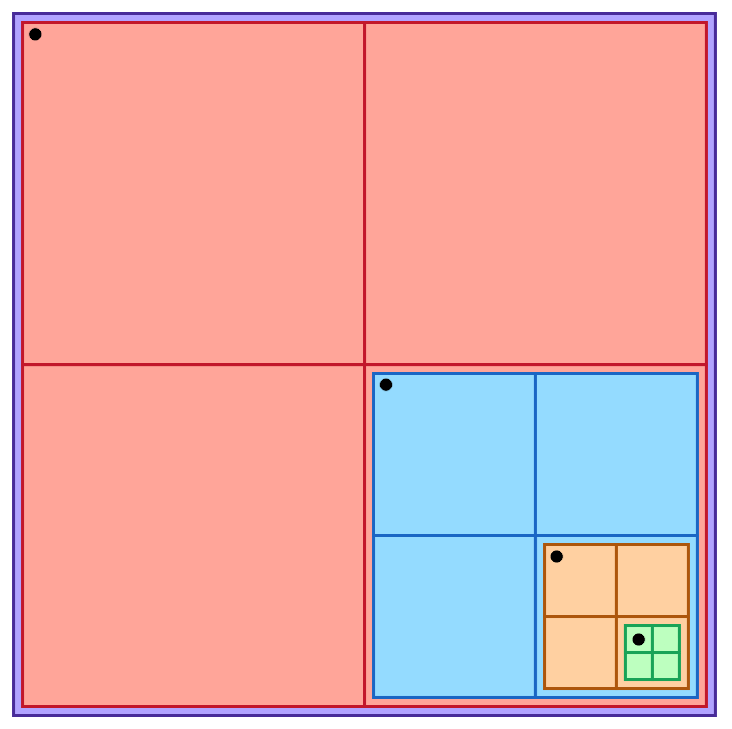
\includegraphics[width=0.35\textwidth]{imgs/worst_case_qb.png}
\caption{An set $X$ where building the Quadtree is manifeslty in $\mathcal{O}(\vert X \vert^2 d)$}
\label{worst_case_qb}
\end{figure}





















\end{document}
